\documentclass[12pt,letterpaper]{article}

\usepackage[utf8]{inputenc}
\usepackage[T1]{fontenc}
\usepackage[spanish]{babel}
\usepackage[margin=2.5cm]{geometry}
\usepackage{graphicx}
\usepackage{booktabs}
\usepackage{array}
\usepackage{caption}
\usepackage{hyperref}
\usepackage{xcolor}
\usepackage{listings}
\usepackage{float}
\usepackage{amsmath}
\usepackage{amssymb}
\usepackage{microtype}
% La expansion de fuente requiere fuentes escalables (no disponibles en EC/CM),
% por lo que solo se usa la protrusion (espaciado optico de margenes).
\microtypesetup{expansion=false}

% Tolerancia para lineas que no pueden justificarse bien (codigo, URLs, etc.)
\setlength{\emergencystretch}{3em}

\hypersetup{
    colorlinks=true,
    linkcolor=blue,
    filecolor=blue,
    urlcolor=blue
}

\captionsetup[figure]{font=small,labelformat=simple,labelsep=period}
\captionsetup[table]{font=small,labelformat=simple,labelsep=period}

\renewcommand{\figurename}{Figura}
\renewcommand{\tablename}{Tabla}

\title{}
\author{}
\date{}

\begin{document}

\begin{titlepage}
    \centering
    \vspace*{2cm}

    {\Large\bfseries Computación de Alto Rendimiento (HPC)\par}
    \vspace{0.5cm}
    {\Large Caso de Estudio 2 --- Concurrencia con OpenMP,\par}
    \vspace{0.2cm}
    {\Large Perfilado y Benchmark\par}

    \vspace{2cm}

    {\Huge\bfseries Paralelización con OpenMP de la\\ multiplicación de matrices,\par}
    \vspace{0.3cm}
    {\Large Caracterización de CPU y memoria, y\\ comparación de rendimiento\\ entre dos máquinas\par}

    \vspace{2cm}

    {\Large
    José Alejandro Quintero Gahona\\[0.3cm]
    Meycol Kleym Quintero Castaño\\[0.3cm]
    María Angélica Alvarez Giraldo\\[0.3cm]
    }

    \vfill

    {\large
    Docente: Ramiro Andrés Barrios Valencia\\[0.3cm]
    Asignatura: Computación de Alto Rendimiento\\[0.3cm]
    \today
    \par}
\end{titlepage}


\newpage
\tableofcontents
\newpage

\section{Introducción y objetivos}

\subsection*{Qué se hizo}

Este documento presenta el caso de estudio 2 de Computación de Alto Rendimiento (HPC). Parte del programa secuencial de multiplicación de matrices del caso de estudio 1 y, sobre él, implementa tres cosas que el enunciado pide:

\begin{enumerate}
    \item \textbf{Concurrencia con OpenMP}, con las directivas elegidas y justificadas a partir de los ejemplos de la especificación oficial.
    \item \textbf{Perfilado de la aplicación} en sus dos ejes mínimos: CPU y memoria.
    \item \textbf{Benchmark en dos máquinas distintas}, con hardware realmente diferente (Intel vs AMD, distinta jerarquía de caché, distinto sistema operativo).
\end{enumerate}

El caso de estudio 1 ya había comparado cuatro estrategias: pthreads, \texttt{fork()} con memoria compartida, optimización de compilación (\texttt{-O3} y variantes) y un kernel transpuesto. Aquí se completa el cuadro con OpenMP como quinta estrategia y, sobre todo, se responde con \textbf{medición} una pregunta que antes era intuición: \textit{¿por qué la transposición de $B$ hace que el kernel sea tan más rápido?}

\subsection*{Objetivos}

\begin{itemize}
    \item Implementar la versión concurrente con OpenMP y justificar técnicamente cada directiva y cláusula utilizada.
    \item Caracterizar la aplicación: dónde se va el tiempo de CPU y qué presión genera sobre la memoria.
    \item Medir el rendimiento en dos máquinas Linux distintas y comparar los resultados.
    \item Integrar las tres mediciones (perfilado, speedup y benchmark) en una explicación única del comportamiento del programa.
\end{itemize}

\subsection*{Organización}

Las secciones 2 y 3 presentan los conceptos y el programa base. La sección 4 describe la implementación con OpenMP. La sección 5 expone el diseño experimental. La sección 6 muestra los resultados, la 7 los analiza y la 8 cierra con las conclusiones.

\section{Objetivos}

\subsection{Objetivo general}

Completar el caso de estudio 2 implementando concurrencia mediante \textbf{OpenMP} sobre la aplicación de multiplicación de matrices, caracterizar el comportamiento de la aplicación a nivel de CPU y de memoria, y medir su rendimiento en dos máquinas diferentes para poder comparar hardware.

\subsection{Objetivos específicos}

\begin{itemize}
    \item Implementar la versión concurrente con \textbf{OpenMP} partiendo del programa secuencial, aplicando las directivas de la API (\texttt{\#pragma omp}) de forma justificada.
    \item Justificar técnicamente la \textbf{elección de cada directiva y cláusula} utilizada, apoyándose en los ejemplos de la especificación oficial de OpenMP.
    \item Realizar el \textbf{perfilado mínimo de la aplicación} en dos ejes: \textbf{CPU} (tiempo por función, con GProf) y \textbf{memoria} (tasa de fallos de caché y footprint de memoria, con Cachegrind y \texttt{getrusage}).
    \item \textbf{Medir el rendimiento en dos máquinas distintas} con Linux, usando un benchmark reproducible, y comparar los resultados mediante la métrica de diferencia porcentual de rendimiento.
    \item Analizar de forma integrada los resultados de \textit{benchmarks}, \textit{profiling} y \textit{speedup} para explicar qué limita el rendimiento de la aplicación.
\end{itemize}

\section{Marco teórico}

En esta sección se introducen los conceptos mínimos necesarios para entender el resto del documento. El objetivo es tener un vocabulario común, no hacer desarrollos matemáticos largos.

\subsection{OpenMP: qué es y qué aporta}

OpenMP es una \textbf{API (Application Programming Interface) diseñada para la computación paralela en arquitecturas de memoria compartida}. No es un lenguaje ni una biblioteca: es un conjunto de \textbf{directivas de compilador}, \textbf{rutinas de biblioteca} y \textbf{variables de ambiente} que permiten al programador describir paralelismo sin escribir explícitamente la creación y sincronización de hilos.

El elemento central es la \textbf{región paralela}. Cuando el hilo maestro encuentra una región paralela, crea un \textit{equipo de hilos} (\textit{team}), todos ejecutan el bloque de código de la región, y al final de la región el hilo maestro espera a que todos terminen. Esa sincronización final es lo que garantiza que los resultados estén listos cuando la ejecución continúa.

La analogía con la versión de pthreads del caso de estudio 1 es directa: allí se escribía a mano el \texttt{pthread\_create} para cada hilo y el \texttt{pthread\_join} para esperarlos. OpenMP hace exactamente eso internamente, pero lo hace el \textit{runtime}.

Tres conceptos gobiernan el comportamiento de una región paralela:

\begin{itemize}
    \item \textbf{Directivas y centinelas}. Una directiva es una línea de código con significado \emph{solo} para el compilador. Se escriben con el centinela \texttt{\#pragma omp}. Un punto fundamental: \textbf{si el programa se compila sin la bandera \texttt{-fopenmp}, las directivas se ignoran silenciosamente} y el código se ejecuta secuencialmente. Por eso el flag de compilación es parte inseparable del uso de OpenMP.
    \item \textbf{Datos compartidos y privados}. En una región paralela, por defecto las variables son \emph{compartidas} (todos los hilos ven la misma copia) salvo las variables de control de los bucles, que son \emph{privadas} por defecto. El programador puede declarar explícitamente qué es compartido y qué es privado con las cláusulas \texttt{shared()} y \texttt{private()}.
    \item \textbf{Sincronización}. La región paralela tiene una \emph{barrier} implícita al final. Además existen construcciones explícitas (\texttt{critical}, \texttt{atomic}, \texttt{barrier}) para cuando varios hilos deben tocar el mismo dato.
\end{itemize}

\subsection{Los tres niveles de un programa paralelo}

En el caso de estudio 1 se implementó la paralelización manual, es decir, el nivel más bajo: el programador decide exactamente qué hace cada hilo. OpenMP introduce un nivel intermedio en el que el programador \emph{describe} qué bucles paralelizar y el \textit{runtime} decide el reparto. Existen además niveles más altos (\textit{tasking}, \textit{worksharing}) que no se usaron en este trabajo.

\subsection{Métricas de rendimiento: MIPS, FLOPS y por qué no sirven aquí}

El \textbf{rendimiento computacional} se puede medir de dos formas distintas:

\begin{itemize}
    \item \textbf{Tiempo de respuesta}: cuánto tarda el sistema en resolver \emph{una} aplicación concreta. Es la métrica del usuario final. Es la que se usa en este trabajo.
    \item \textbf{Throughput (productividad)}: cuánto trabajo es capaz de completar el sistema en un intervalo de tiempo. Es una métrica del \emph{sistema}, más cercana a la de un servidor con many workloads.
\end{itemize}

Para comparar dos máquinas se define el rendimiento como $R = 1/T$ y la diferencia porcentual:

\[
\%\Delta = \frac{R_x - R_y}{R_y} \times 100
\]

Las unidades de medida históricas para cuantificar el rendimiento computacional son:

\begin{itemize}
    \item \textbf{MIPS} (millions of instructions per second):Instructions per second. Es la unidad clásica, pero \textbf{depende fuertemente del repertorio de instrucciones} de cada microarquitectura, por lo que es poco comparable entre arquitecturas distintas.
    \item \textbf{FLOPS} (floating point operations per second): operaciones de coma flotante por segundo. Es la unidad moderna y se usa en el ranking \textit{Top500}. El problema es que \textbf{solo aplica a operaciones de coma flotante}.
\end{itemize}

En este trabajo el kernel trabaja con \textbf{enteros}, por lo que \textbf{no se puede reportar la aplicación en FLOPS}. Esta es una limitación real y no un descuido: la alternativa sería reescribir el kernel con \texttt{double}, lo que cambiaría el objeto de estudio (el algoritmo de punto flotante tiene sus propios problemas de precisión y de uso de la FPU) sin aportar nada a la pregunta que se quiere responder. Por eso se reportan \textbf{tiempos, speedup y diferencia porcentual de rendimiento}, que además es lo que el enunciado de la actividad pide de forma explícita.

\subsection{Benchmark: definición y tipos}

Un \textbf{benchmark} es un programa que permite evaluar el rendimiento de una arquitectura o de un equipo. Su lógica es generar una \emph{carga de trabajo} conocida y estandarizada para la cual se puede predecir el rendimiento en un trabajo real.

Según la procedencia de la carga de trabajo, los benchmarks se clasifican en:

\begin{itemize}
    \item \textbf{Programas reales completos}: por ejemplo un compilador, un procesador de textos, un outil CAD. Son los más representativos.
    \item \textbf{Kernels extraídos de programas reales}: es la categoría de este trabajo. Se extrae la parte central (el \textit{kernel}) de un programa real que es la que consume la mayor parte del tiempo de ejecución. El profesor insistió en medir el tiempo del \emph{kernel} de la multiplicación de matrices, no el programa completo, porque es el kernel lo que domina el tiempo y lo que determina el comportamiento de la caché.
    \item \textbf{Programas reducidos o \textit{toys}}: programas muy pequeños, de 10 a 100 líneas, que generan carga sin resolver un problema real.
    \item \textbf{Programas sintéticos}: creados artificialmente para generar carga en un recurso específico.
\end{itemize}

Una advertencia importante del profesor: los benchmarks reducidos y los sintéticos \textbf{no cargan la memoria principal de forma realista}, por lo que no son una buena opción para caracterizar el desempeño de una aplicación real. Para eso hay que usar programas reales o \emph{kernels} extraídos de problemas reales, como el nuestro.

\subsection{Perfilado: definición y tipos}

El \textbf{perfilado} (\textit{profiling}) tiene un objetivo distinto al benchmark. El benchmark mide el \emph{desempeño}; el perfilado busca \textbf{identificar el comportamiento del programa en una arquitectura específica}: dónde están los puntos ineficientes, dónde hay embotellamiento de memoria o de acceso a disco, y qué explica el escalamiento de la solución.

Las herramientas de perfilado se clasifican por su mecanismo:

\begin{itemize}
    \item \textbf{Contadores de hardware}: leen directamente los contadores del procesador (ciclos, instrucciones, fallos de caché).
    \item \textbf{Muestreo (\textit{sampling})}: interrumpen el programa en intervalos periódicos y capturan el estado, para después hacer un análisis estadístico. Es el mecanismo de \texttt{perf} y de \texttt{gprof}.
    \item \textbf{Trazado (\textit{tracing})}: en lugar de interrumpir periódicamente, detectan la ocurrencia de un evento concreto (por ejemplo, una llamada a función) y lo registran.
\end{itemize}

En este trabajo se usan dos herramientas, que cubren los dos ejes pedidos por la consigna:

\begin{itemize}
    \item \textbf{GProf}: perfilador por muestreo que se integra con el compilador. Se activa con la bandera \texttt{-pg}, que inserta instrumentación en el programa. Al ejecutarse, el programa escribe un archivo \texttt{gmon.out} con los contadores recolectados; luego la utilidad \texttt{gprof} convierte ese archivo binario en un reporte legible. Es la herramienta que el profesor presentó en clase.
    \item \textbf{Cachegrind}: perfilador de simulación de caché, parte de Valgrind. Reproduce el comportamiento de una jerarquía de caché (L1, LL) durante la ejecución y reporta, para cada función, cuántas instrucciones se ejecutaron y cuántas fallaron en caché. Con la opción \texttt{--cache-sim=yes} reporta además las tasas de fallo (\textit{miss rate}) de lectura y escritura.
\end{itemize}

\subsection{La jerarquía de caché y el miss rate}

El procesador no accede directamente a la memoria RAM: hay una jerarquía de cachés, pequeños y muy rápidos, entre el núcleo y la RAM.

\begin{center}
\begin{tabular}{|l|c|c|}
\hline
\textbf{Nivel} & \textbf{Tamaño típico} & \textbf{Tiempo de acceso} \\
\hline
L1 (datos e instrucciones) & 32--64 KiB por núcleo & ~4 ciclos \\
L2 & 512 KiB--2 MiB por núcleo & ~12 ciclos \\
L3 (compartida) & 8--32 MiB & ~40 ciclos \\
RAM & GiB & ~200 ciclos \\
\hline
\end{tabular}
\end{center}

El \textbf{miss rate} es la fracción de accesos a un nivel de caché que no se encuentran en ese nivel y deben bajar al nivel inferior. Es la métrica clave para entender el rendimiento de un kernel: un miss a RAM cuesta cientos de ciclos, mientras que un acierto a L1 cuesta unos pocos.

Cuando se dice que un acceso es \emph{contiguo} o \emph{secuencial}, se está describiendo el patrón con que se recorre un arreglo en memoria. En el algoritmo clásico de multiplicación de matrices, el acceso a $B$ no es contiguo, y esa es la raíz del problema que se mide en la sección 8.

\section{El programa base (versión secuencial)}

\subsection{Qué hace el programa}

El programa toma dos matrices cuadradas $A$ y $B$ de tamaño $N \times N$ y calcula la matriz producto $C = A \times B$ con el algoritmo clásico. Cada elemento se calcula como:

\[
C[i][j] = \sum_{k=0}^{N-1} A[i][k] \cdot B[k][j]
\]

Hay $N^2$ elementos a producir y cada uno requiere $N$ multiplicaciones y $N-1$ sumas, así que la complejidad es $O(N^3)$. Para $N = 1000$ son $10^9$ operaciones; para $N = 4000$, $6.4 \times 10^{10}$.

\subsection{El algoritmo en código}

El bucle que después se paraleliza en todas las versiones es un triple bucle anidado:

\begin{verbatim}
for (int i = 0; i < N; i++)
    for (int j = 0; j < N; j++)
        for (int k = 0; k < N; k++)
            C[i*N + j] +=
                A[i*N + k] *
                B[k*N + j];
\end{verbatim}

Los índices \texttt{i*N + k} y \texttt{k*N + j} convierten el índice bidimensional \texttt{[i][k]} en uno unidimensional \texttt{[i*N+k]}, porque las matrices se almacenan en un bloque contiguo de memoria (allocado con \texttt{malloc}), no como arreglos bidimensionales de C.

\subsection{El patrón de acceso a memoria}

Este es el detalle que resultará central en el análisis, así que conviene hacerlo explícito desde el inicio. En el bucle interior, con $i$ y $j$ fijos, el índice \texttt{k} recorre:

\begin{itemize}
    \item $A[i \cdot N + k]$: acceso \textbf{contiguo}. Al avanzar $k$, la dirección avanza de a un entero. La fila $i$ de $A$ se recorre secuencialmente.
    \item $B[k \cdot N + j]$: acceso \textbf{con salto}. Al avanzar $k$, la dirección avanza $N$ enteros. La columna $j$ de $B$ se recorre \emph{a saltos}, y cada salto de $N$ enteros cae normalmente en una línea de caché diferente.
    \item $C[i \cdot N + j]$: acceso \textbf{constante}. Todos los $k$ escriben en la misma celda, que queda en un registro.
\end{itemize}

Es decir: la mitad del trabajo de la multiplicación (la lectura de $B$) accede a la memoria en un orden que no corresponde al orden en que los datos están almacenados. Este patrón es el que se mide en la sección 8 con Cachegrind y el que explica, en la sección 11, por qué la transposición de $B$ produce una ganancia tan grande sin necesidad de paralelizar.

\subsection{Estructura modular del código}

El proyecto está organizado en módulos, de manera que el kernel de multiplicación (que es lo que cambia entre versiones) está aislado del resto:

\begin{itemize}
    \item \texttt{modules/memoria.c}: reserva memoria para las tres matrices con \texttt{malloc} y verifica que la reserva haya sido exitosa.
    \item \texttt{modules/llenado.c}: llena $A$ y $B$ con valores aleatorios usando \texttt{srand}/\texttt{rand} y pone $C$ en cero.
    \item \texttt{modules/tiempo\_mult.c}: contiene la función \texttt{multiplicar\_y\_medir} que ejecuta el triple bucle secuencial y mide el tiempo con \texttt{clock\_gettime}.
    \item \texttt{modules/tiempo\_mult\_trans.c}: variante con $B$ transpuesta, que accede a $B$ por fila.
    \item \texttt{modules/tiempo\_mult\_openmp.c}: variante con la directiva \texttt{\#pragma omp parallel for collapse(2)}, que es la implementación de este caso de estudio.
    \item \texttt{src/matriz\_monotonic\_openmp.c}: programa principal que usa el kernel con OpenMP.
\end{itemize}

El \textit{headers} correspondientes viven en \texttt{include/}. Esta separación permite medir el \emph{kernel} de forma aislada, que es lo que interesa para el perfilado.

\section{Medición del tiempo}

\subsection{Wall clock vs tiempo de CPU}

En cualquier sistema operativo hay dos formas de medir cuánto tarda un programa:

\begin{itemize}
    \item \textbf{Wall clock}: el tiempo total transcurrido desde que el programa arranca hasta que termina. Es lo que un usuario percibe como ``cuánto tardó''. Incluye las esperas por E/S, las pausas por quantum y cualquier otra cosa que pase en el sistema.
    \item \textbf{Tiempo de CPU}: el tiempo que la CPU pasó efectivamente ejecutando nuestro programa. Se subdivide en tiempo de \textbf{usuario} (código nuestro) y tiempo de \textbf{sistema} (atendiendo llamadas al kernel).
\end{itemize}

Durante la materia, el profesor indicó que la métrica correcta para comparar rendimiento entre programas es el \textbf{wall clock}, porque refleja la experiencia real del usuario. El tiempo de CPU mide otra cosa (cuánto trabajó el procesador), pero no cuánto tardó el programa en completarse. En este trabajo se mide con wall clock en todos los casos.

\subsection{Qué opciones hay en C}

El lenguaje C ofrece varias funciones de tiempo. Esta tabla resume las que se consideraron:

\begin{center}
\scriptsize
\begin{tabular}{|l|l|c|}
\hline
\textbf{Función} & \textbf{Qué mide} & \textbf{Wall clock?} \\
\hline
\texttt{clock()} & Tiempo de CPU & \textcolor{red}{No} \\
\texttt{timespec\_get}\newline\texttt{(TIME\_UTC)} & Wall clock, pero afectado por cambios de hora & \textcolor{red}{No (frágil)} \\
\texttt{clock\_gettime}\newline\texttt{(CLOCK\_MONOTONIC)} & Wall clock monotónico & \textcolor{green}{Sí} \\
\texttt{clock\_gettime}\newline\texttt{(CLOCK\_MONOTONIC\_RAW)} & Wall clock, sin ajustes de NTP & \textcolor{green}{Sí, mejor} \\
\hline
\end{tabular}
\end{center}

\subsection{Por qué \texttt{CLOCK\_MONOTONIC\_RAW}}

De las cuatro, \texttt{clock\_gettime(CLOCK\_MONOTONIC\_RAW)} ofrece las mejores garantías para benchmarking:

\begin{itemize}
    \item Es \textbf{monotónica}: nunca devuelve un valor menor que el anterior, aunque se cambie la hora del sistema manualmente.
    \item Es \textbf{raw} (cruda): no se ve afectada por los ajustes graduales que NTP hace al reloj del sistema para sincronizarlo con servidores de hora externos. Estos ajustes pueden sumar o restar microsegundos al reloj, lo que introduce ruido en mediciones de corta duración.
\end{itemize}

\subsection{Qué se cronometra y qué no}

Se cronometra \textbf{solo el trabajo de multiplicación}. La reserva de memoria, la generación de las matrices aleatorias y la impresión de resultados quedan fuera del tiempo medido, porque no son el trabajo que estamos analizando. Esto tiene una consecuencia relevante para el perfilado: la función que contiene el triple bucle es la que domina el tiempo, y por eso es la que aparece en el reporte de GProf con el 100\% del tiempo propio.

\subsection{Por qué se repite el experimento 10 veces}

Una sola medición no es estadísticamente confiable: el sistema operativo puede tener otras tareas corriendo, una preempción puede caer justo en la corrida, o un proceso del sistema puede usar la CPU en el momento crítico. Para aislar este \textbf{ruido del sistema} se repite el experimento 10 veces por configuración y se calcula:

\begin{itemize}
    \item \textbf{Media} aritmética: el promedio de las 10 mediciones.
    \item \textbf{Mediana}: el valor central al ordenar las 10 mediciones. Es \textbf{robusta} frente a valores atípicos.
    \item \textbf{Desviación estándar} ($\sigma$): qué tanto se dispersan las mediciones.
\end{itemize}

En este trabajo se usa la \textbf{mediana} como estimador central del speedup, por la misma razón que en el caso de estudio 1.

\subsection{El orden de los bucles importa}

El script que ejecuta el experimento recorre las repeticiones por fuera y los tamaños por dentro:

\begin{verbatim}
for cada_T:
  for repeticion in 1..10:
    for cada_N:
      medir(N, T)
\end{verbatim}

El profesor explicó que si las 10 repeticiones de un mismo tamaño se hicieran seguidas, los datos quedarían \textit{calientes} en la caché del procesador y la medición saldría artificialmente rápida. Al intercalar tamaños entre repeticiones, cada medición se ve forzada a trabajar con datos nuevos en RAM, dando un resultado más realista.

\section{Implementación con OpenMP}

\subsection{Del diseño manual al declarativo}

En el caso de estudio 1 la paralelización con pthreads se hizo \emph{a mano}: el programa calculaba los rangos de filas de cada hilo, creaba los $T$ hilos con \texttt{pthread\_create}, y esperaba con \texttt{pthread\_join}. Con OpenMP no se escribe nada de eso: se declara qué bucle se paraleliza y el \textit{runtime} se encarga del resto.

El punto de partida fue, como pidió el profesor, la \textbf{versión secuencial inicial}. El kernel con OpenMP vive en su propio módulo (\texttt{modules/tiempo\_mult\_openmp.c}) y el programa principal (\texttt{src/matriz\_monotonic\_openmp.c}) es una copia del secuencial con dos cambios: incluir el header del kernel nuevo y llamar a \texttt{multiplicar\_y\_medir\_openmp}.

\subsection{La directiva elegida}

El pragma que se aplica al triple bucle es:

\begin{verbatim}
#pragma omp parallel for collapse(2)
for (int i = 0; i < N; i++) {
    for (int j = 0; j < N; j++) {
        for (int k = 0; k < N; k++) {
            C[(size_t)i * N + j] +=
                A[(size_t)i * N + k] *
                B[(size_t)k * N + j];
        }
    }
}
\end{verbatim}

\subsection{Justificación a partir de los ejemplos de la especificación}

Antes de escribir el código se revisaron los ejemplos del documento oficial \textit{OpenMP Application Programming Interface Examples v6.0.1} (disponible en \texttt{github.com/OpenMP/Examples}), siguiendo la indicación del profesor de no escoger las directivas al azar sino escogerlas entendiendo. Del índice, tres ejemplos son aplicables al patrón del kernel:

\begin{center}
\begin{tabular}{|l|p{6cm}|p{6cm}|}
\hline
\textbf{Ejemplo} & \textbf{Patrón} & \textbf{Veredicto} \\
\hline
\textbf{3.1} \texttt{ploop.1.c} &
\texttt{\#pragma omp parallel for} sobre un solo loop &
Solo paraleliza el loop externo $i$. Con $N=4000$ eso da 4000 bloques de trabajo, mal repartidos entre 12 núcleos. \\
\hline
\textbf{3.8} \texttt{collapse.1.c} &
\texttt{\#pragma omp for collapse(2)} sobre dos loops anidados &
\textbf{Elegido.} Une $i$ y $j$ en un único espacio de $N^2$ iteraciones (16 millones para $N=4000$) con buen reparto entre hilos. \\
\hline
\textbf{5.3.5} \texttt{task\_dep.5.c} &
\texttt{\#pragma omp task depend(in/inout)} sobre bloques &
Descartado. Asume un kernel bloqueado y el cálculo explícito de dependencias entre bloques; es más complejo de lo que el caso requiere. \\
\hline
\end{tabular}
\end{center}

\subsection{Por qué cada elemento de la directiva}

\begin{itemize}
    \item \textbf{\texttt{parallel for} (combinada)}: crea el equipo de hilos y reparte el trabajo del loop en una sola directiva. Es más limpio que separar \texttt{\#pragma omp parallel} de \texttt{\#pragma omp for}, y el ejemplo 3.1 del PDF muestra las dos formas equivalentes.
    \item \textbf{\texttt{collapse(2)}}: es la clave de la elección. \emph{Colapsar} dos loops anidados significa que el \textit{runtime} los trata como un único espacio de iteraciones de tamaño $N \times N$, y reparte ese espacio entre los hilos. Sin \texttt{collapse}, solo se paralelizaría el loop $i$, y con $N=2000$ eso daría 2000 bloques para 12 núcleos: un reparto muy desigual, con hilos excediendo en carga y otros esperando. El loop $k$ queda secuencial dentro de cada par $(i,j)$, que es lo correcto, porque la acumulación del producto punto debe permanecer en un solo hilo.
    \item \textbf{No se usa \texttt{private(k)} explícito}: en C99 las variables de control de un \texttt{for} ya son implícitamente privadas dentro de un loop construct. Declararlo explícitamente además \emph{falla la compilación}, porque $k$ está declarada dentro del \texttt{for} y por tanto no es visible en el punto donde aparece la directiva.
\end{itemize}

\subsection{Por qué no se necesitan otras cláusulas}

Este es el punto donde el conocimiento del algoritmo es lo que garantiza la corrección:

\begin{itemize}
    \item $A$, $B$ y $C$ quedan \textbf{shared} por defecto, y eso es lo correcto: $A$ y $B$ solo se leen, y cada hilo solo escribe en $C[i \cdot N + j]$ para el par $(i,j)$ concreto que le tocó en el espacio colapsado.
    \item \textbf{No hace falta \texttt{reduction(+:)}}. Una \textit{reduction} se usa cuando varios hilos acumuran sobre la \emph{misma} variable. Aquí cada $C[i][j]$ es acumulado íntegramente por un solo hilo (el que posee ese par $(i,j)$), y los hilos distintos escriben en celdas distintas. No hay conflicto.
    \item \textbf{No hace falta \texttt{critical} ni \texttt{atomic}}. No existe región crítica: no hay ninguna variable compartida que se modifique de forma no determinista.
    \item \textbf{No hace falta \texttt{barrier}} explícita. La región paralela ya tiene una barrera implícita al final, que garantiza que todos los hilos terminaron antes de que el programa principal imprima los resultados.
\end{itemize}

\subsection{Configuración del número de hilos}

El número de hilos con el que corre la región paralela se puede fijar en tres lugares, por orden de precedencia:

\begin{enumerate}
    \item La cláusula \texttt{num\_threads()} de la propia directiva.
    \item La llamada a \texttt{omp\_set\_num\_threads()}.
    \item La variable de ambiente \texttt{OMP\_NUM\_THREADS}.
\end{enumerate}

En este trabajo se usa la variable de ambiente \texttt{OMP\_NUM\_THREADS}, que es la forma más portable y la que además permite barrer el número de hilos \emph{sin recompilar} el binario. Es la misma estrategia que mostró el profesor en clase al cambiar de 8 a 4 hilos y ver cómo cambiaba el comportamiento del programa.

\subsection{El flag de compilación no es opcional}

Un detalle fundamental de OpenMP: \textbf{las directivas se ignoran silenciosamente si no se compila con \texttt{-fopenmp}}. El programa compilaría sin errores, se ejecutaría, y daría exactamente el mismo resultado secuencial. Por eso el flag es parte del diseño y no un detalle de invocación.

Además, hay que cuidar que el flag de optimización sea el \textbf{mismo que usan las demás estrategias} de la comparación. En una primera versión de este trabajo el binario de OpenMP se compiló con \texttt{-O0} mientras que el resto de estrategias usaban \texttt{-O2}; esa diferencia hacía que el speedup de OpenMP pareciera artificialmente malo (entre 0.71$\times$ y 1.48$\times$), porque la comparación mezclaba dos efectos distintos: el paralelismo y la ausencia de optimización del compilador. Con \texttt{-fopenmp -O2}, el $T=1$ de OpenMP da 76.02\,s contra los 75.65\,s del secuencial con \texttt{-O2}: una diferencia del 0.5\%, que confirma que la base de comparación quedó justa.

\section{Benchmark: protocolo y marco de comparación}

\subsection{Qué se mide y por qué el kernel}

La consigna pide medir el rendimiento de la aplicación en dos máquinas diferentes. Como se explicó en la sección 3, un benchmark debe generar una carga \emph{representativa}. En este trabajo la carga representativa es \textbf{el kernel de la multiplicación de matrices}, por dos razones:

\begin{enumerate}
    \item Es lo que consume la mayor parte del tiempo de ejecución del programa (el 100\% del tiempo propio según el perfil de GProf, sección 8), por lo que es el componente que determina el comportamiento del hardware.
    \item Es el componente \emph{reproducible}: dada la misma semilla, genera exactamente los mismos datos en cualquier equipo, lo que hace comparables las mediciones entre máquinas.
\end{enumerate}

Las otras fases del programa (reservar memoria, llenar las matrices con números aleatorios, imprimir) quedan fuera del cronometrado, de la misma manera que en el caso de estudio 1.

\subsection{Qué se compara entre las dos máquinas}

Para cada máquina se mide:

\begin{itemize}
    \item El \textbf{tiempo de ejecución} del kernel con OpenMP, con el mismo barrido de parámetros: $T \in \{1, 2, 4, 8, 16\}$ y $N \in \{500, 1000, 2000, 4000\}$, 10 repeticiones por combinación.
    \item El \textbf{speedup interno} de cada máquina: $S = T_{T=1} / T_{T}$, es decir, cuánto acelera su propio paralelismo.
    \item La \textbf{diferencia porcentual de rendimiento} entre máquinas, con la fórmula de la sección 3:
    \begin{equation}
    \%\Delta = \frac{R_x - R_y}{R_y} \times 100, \qquad R = \frac{1}{T}
    \end{equation}
\end{itemize}

El \textbf{speedup interno} es la métrica más informativa para comparar máquinas, porque es \emph{independiente de la velocidad bruta del equipo}: mide cuánto paralelismo es capaz de extraer cada hardware. Un equipo más lento puede tener mejor speedup si su memoria es más rápida o si tiene menos núcleos que disputan la caché.

\subsection{El protocolo para garantizar comparabilidad}

Un benchmark entre máquinas solo es válido si las condiciones son equivalentes. El protocolo que se siguió en ambas máquinas:

\begin{itemize}
    \item \textbf{Mismo código fuente}: la misma rama del repositorio, verificada con el mismo hash de commit.
    \item \textbf{Mismos flags de compilación}: \texttt{-Wall -O2 -fopenmp} en ambos equipos, y el mismo compilador cuando es posible (\texttt{gcc}).
    \item \textbf{Mismos datos}: semilla 42 y valor máximo 9 en todas las corridas, por lo que las matrices son idénticas bit a bit.
    \item \textbf{Misma methodology de repetición}: 10 corridas por configuración, intercalando los tamaños de matriz (ver sección 5) y usando la mediana.
    \item \textbf{Mismo estado del equipo}: sin otras cargas, con el equipo conectado a la corriente (para que el procesador no baje su frecuencia) y con la temperatura estable.
\end{itemize}

\subsection{Qué se captura del hardware}

Para poder interpretar los resultados, de cada equipo se registra automáticamente la información relevante:

\begin{center}
\begin{tabular}{|l|p{9cm}|}
\hline
\textbf{Dato} & \textbf{Para qué sirve} \\
\hline
Modelo de CPU y familia & Determina el conjunto de instrucciones y el rendimiento por ciclo \\
Núcleos físicos y lógicos & Explica el techo de paralelismo y la capacidad de la caché compartida \\
Jerarquía de caché (L1d, L2, L3) & Explica el comportamiento de la caché del kernel \\
Frecuencia máxima y mínima & Explica la variabilidad del rendimiento \\
Memoria RAM & Limita el $N$ máximo y el comportamiento del ancho de banda de memoria \\
Kernel y distribución & Explica diferencias en el comportamiento del sistema \\
Versión del compilador & Explica diferencias en el código generado \\
\hline
\end{tabular}
\end{center}

\section{Perfilado de la aplicación}

\subsection{Objetivo del perfilado}

El perfilado responde una pregunta distinta a la del benchmark. El benchmark mide \emph{cuánto}; el perfilado busca \textbf{explicar por qué}. Concretamente, en este trabajo se busca:

\begin{enumerate}
    \item Identificar \textbf{dónde se va el tiempo de CPU} de la aplicación (perfilado de CPU).
    \item Identificar \textbf{cuánta presión sobre la memoria} genera el kernel y si el acceso a la caché es eficiente (perfilado de memoria).
    \item Explicar el \textbf{escalamiento} observado: por qué el speedup con OpenMP es alto pero no se acerca al ideal, y por qué la transposición de $B$ produce una ganancia mayor que la paralelización.
\end{enumerate}

\subsection{Perfilado de CPU con GProf}

GProf es un perfilador por \textbf{muestreo} que se integra con el compilador. El procedimiento, tal como lo presentó el profesor, tiene tres pasos:

\begin{enumerate}
    \item \textbf{Compilar con instrumentación}: la bandera \texttt{-pg} le indica al compilador que inserte llamadas a funciones de conteo en el programa.
    \item \textbf{Ejecutar}: el programa instrumentado corre normalmente y al terminar escribe un archivo \texttt{gmon.out} con los contadores recolectados.
    \item \textbf{Generar el reporte}: \texttt{gprof binario gmon.out} convierte ese archivo binario en un reporte legible en texto plano.
\end{enumerate}

El reporte contiene el \emph{flat profile}, donde cada función aparece con el porcentaje de tiempo propio, los segundos acumulados, el número de llamadas y el tiempo medio por llamada.

Se aplicó a las tres variantes del kernel: secuencial, transpuesta y con OpenMP. Hay una \textbf{limitación importante con OpenMP}: GProf solo instrumenta el hilo principal, de modo que el tiempo de la región paralela se contabiliza de forma engañosa (aparece atribuido a la función que la contiene y no a la función de trabajo real). Por eso el reporte de GProf es concluyente para las variantes secuenciales y se reporta con la advertencia explícita para la variante con OpenMP.

\subsection{Perfilado de memoria con Cachegrind}

Para el eje de memoria se usó \textbf{Cachegrind}, la herramienta de simulación de caché que forma parte de Valgrind. Cachegrind reproduce el comportamiento de una jerarquía de caché durante la ejecución y reporta, para el programa completo y para cada función:

\begin{itemize}
    \item \textbf{Instrucciones ejecutadas} (\textit{I refs}).
    \item \textbf{Referencias a datos} (\textit{D refs}), separadas en lecturas y escrituras.
    \item \textbf{Fallos de caché} (\textit{misses}) en L1 de datos (\textit{D1}) y en el último nivel (\textit{LL}).
    \item \textbf{Tasa de fallo} (\textit{miss rate}) de lectura y de escritura.
\end{itemize}

Para activar la simulación de caché hay que pasar la opción \texttt{--cache-sim=yes}; sin ella Cachegrind solo reporta el conteo de instrucciones.

Valgrind no venía instalado en el sistema, pero no hizo falta permiso de administrador: el script \texttt{experiments/bootstrap\_tools.sh} descarga el paquete con \texttt{apt-get download} (que no requiere \texttt{sudo}) y lo extrae con \texttt{dpkg-deb -x} en una carpeta local del proyecto, ajustando la variable \texttt{VALGRIND\_LIB} para que encuentre sus archivos de soporte.

\subsection{Footprint de memoria con \texttt{getrusage}}

Para completar el eje de memoria con la medida del \emph{tamaño} del espacio de memoria utilizado (y no solo su eficiencia), se midió el \textbf{max RSS} (\textit{maximum resident set size}), que es la cantidad máxima de memoria física que el proceso tuvo residente simultáneamente. Se obtuvo con la llamada al sistema \texttt{getrusage(RUSAGE\_CHILDREN, ...)}, envuelta en un pequeño programa auxiliar (\texttt{experiments/maxrss.c}) que ejecuta la aplicación y reporta el pico de memoria del hijo. Esta medida no depende de ninguna herramienta externa.

\subsection{Alcance del perfilado}

El perfilado \textbf{caracteriza la aplicación}: dice dónde se va el tiempo y cuánta presión sobre la memoria genera el kernel. El perfilado de CPU (GProf) se corre en las dos máquinas, mientras que el detalle fino de caché (Cachegrind) se midió en la máquina A, que es donde se corrió el experimento de desempeño principal.

La comparación entre las dos máquinas se hace por otra vía: con el \textbf{benchmark}, que sí se ejecutó en los dos equipos (sección de comparación entre máquinas).

\subsection{Tamaño de N usado para el perfilado}

Cachegrind simula la caché instrucción por instrucción, lo que lo hace entre 50 y 100 veces más lento que la ejecución nativa. Por eso el perfilado se hizo con $N = 500$ en lugar de $N = 4000$. Esta limitación es aceptable: la \emph{tasa} de fallo de caché es una propiedad del \emph{patrón de acceso}, y el patrón de acceso del kernel es el mismo para cualquier $N$ (solo cambia la cantidad de trabajo). Es más, se verificó que la tasa de fallo se mantiene estable entre $N = 500$ y $N = 1000$.

\section{Diseño experimental}

\subsection{Variables}

\begin{itemize}
    \item \textbf{Tamaño de la matriz} ($N$): 500, 1000, 2000 y 4000. Se eligió un rango con saltos de factor 2, desde problemas chicos (donde el paralelismo es marginal) hasta problemas grandes (donde el paralelismo muestra todo su potencial).
    \item \textbf{Cantidad de hilos} ($T$): 1 (secuencial), 2, 4, 8 y 16. Se usa exactamente el mismo conjunto que en la rama de pthreads del caso de estudio 1, para que las curvas sean directamente comparables.
    \item \textbf{Variable medida}: tiempo de la multiplicación en segundos, con \texttt{clock\_gettime} y \texttt{CLOCK\_MONOTONIC\_RAW}.
    \item \textbf{Métricas calculadas}: \textit{speedup} contra el secuencial, tasa de fallo de caché (\textit{miss rate}), número de instrucciones ejecutadas y memoria máxima residente (\textit{max RSS}).
\end{itemize}

En total se ejecutan \textbf{200 mediciones de desempeño} por máquina (5 valores de $T$ × 4 valores de $N$ × 10 repeticiones), más las 5 corrida de Cachegrind y las 5 de \texttt{getrusage} del perfilado.

\subsection{Metodología: 10 corridas por configuración}

Para cada combinación de $T$ y $N$ se ejecutan \textbf{10 corridas independientes} y se calcula la mediana. Como se explicó en la sección 5, una sola medición no es confiable por el ruido del sistema, y la mediana es el estimador robusto frente a valores atípicos.

\subsection{Orden de los bucles}

El script que automatiza el experimento recorre las repeticiones por fuera y los tamaños por dentro, de forma que las 10 repeticiones de un mismo $N$ no queden consecutivas. El motivo ya se explicó: evita que los datos queden \textit{calientes} en la caché y que la medición salga artificialmente rápida.

\subsection{Correctitud: validación contra una implementación de referencia}

Medir tiempos sin verificar que el programa calcula lo correcto es un error metodológico grave. Por eso, antes de cada corrida de medición, el script \texttt{experiments/medir\_openmp.sh} ejecuta una \textbf{validación de correctitud}:

\begin{enumerate}
    \item Se genera con \texttt{experiments/verify\_ref} una matriz resultado de referencia con $N=10$ y semilla 42, usando una implementación ingenua de tres bucles anidados.
    \item Se ejecuta el binario de OpenMP con los mismos parámetros ($N=10$, valor máximo 9, semilla 42).
    \item Se comparan las dos matrices $C$ elemento a elemento.
    \item Si \textbf{no coinciden exactamente}, el script aborta con un mensaje de error y no se mide nada.
\end{enumerate}

El mecanismo es el mismo que se usó en los labs 1 y 2 del caso de estudio 1, y por eso la implementación de referencia (\texttt{experiments/verify\_ref.c}) se reutilizó sin modificaciones.

\subsection{Reproducibilidad del benchmark entre máquinas}

El benchmark entre equipos se automatizó con \texttt{experiments/bench.sh}, que es un script \emph{portable}: corre en cualquier equipo con Linux sin necesidad de nada instalado que no venga de base, y produce un archivo de resultados con el hardware detectado más las corridas crudas. La guía completa para ejecutarlo en el segundo equipo está en \texttt{experiments/REPRODUCIR\_OTRA\_MAQUINA.md}.

\subsection{Herramientas}

\begin{center}
\begin{tabular}{|l|p{8.5cm}|}
\hline
\textbf{Herramienta} & \textbf{Uso en este trabajo} \\
\hline
\texttt{gcc} 14.2.0 & Compilador. Flag \texttt{-Wall -O2 -fopenmp}. \\
\texttt{gprof} & Perfilado de CPU por muestreo con instrumentación \texttt{-pg}. \\
\texttt{valgrind}/\texttt{cachegrind} & Perfilado de memoria: simulación de caché, D1/LL misses. \\
\texttt{getrusage} & Memoria máxima residente (max RSS) del proceso hijo. \\
\texttt{lscpu}, \texttt{free}, \texttt{uname} & Captura automática del hardware de cada equipo. \\
\texttt{matplotlib} & Generación de las gráficas de los resultados. \\
\hline
\end{tabular}
\end{center}

\section{Resultados}

En esta sección se muestran los tres conjuntos de resultados: el perfilado de la aplicación, el desempeño de OpenMP frente a las demás estrategias y la comparación entre las dos máquinas. Todos los tiempos están en segundos y, cuando corresponde, se reporta la \textbf{mediana} de las 10 corridas.

\subsection{Perfilado de CPU: dónde se va el tiempo}

El reporte de GProf para el kernel secuencial es concluyente:

\begin{center}
\begin{tabular}{|l|r|r|r|}
\hline
\textbf{Función} & \textbf{\% tiempo propio} & \textbf{llamadas} & \textbf{ms/llamada} \\
\hline
\texttt{multiplicar\_y\_medir} & 100.13 & 1 & 140.19 \\
\texttt{llenar\_matrices\_con\_semilla} & 0.00 & 1 & 0.00 \\
\texttt{reservar\_matrices} & 0.00 & 1 & 0.00 \\
\hline
\end{tabular}
\end{center}

El 100\% del tiempo propio de la aplicación está en la función del kernel de multiplicación, y el relleno de las matrices y la reserva de memoria son marginales. Esto confirma la decisión metodológica de cronometrar solo el kernel: es la única parte que importa.

\begin{quote}
\textbf{Advertencia sobre GProf con OpenMP.} GProf solo instrumenta el hilo principal. En la variante con OpenMP el tiempo de la región paralela se contabiliza de forma engañosa (aparece atribuido a la función que crea el equipo de hilos, no a la de trabajo real). Por eso el reporte de la variante paralela no se usa para extraer conclusiones sobre el reparto de trabajo entre hilos; para eso están los datos de Cachegrind.
\end{quote}

\subsection{Perfilado de memoria: el comportamiento de la caché}

Esta es la medición más relevante del trabajo, porque cuantifica la hipótesis que el caso de estudio 1 dejó solo como intuición. La tabla~\ref{tab:cachegrind} muestra los contadores de Cachegrind para las tres variantes del kernel, con $N=500$, medidos en la \textbf{máquina A} (Intel Core i5-12450HX, L1d de 40\,KiB por núcleo con 8 vías, L3 compartido de 12\,MiB).

\begin{table}[ht]
\centering
\scriptsize
\begin{tabular}{|l|c|r|r|r|r|r|}
\hline
\textbf{Variante} & \textbf{T} & \textbf{I refs} & \textbf{D refs} & \textbf{D1 misses} & \textbf{D1 miss rate (lect.)} & \textbf{LLd misses} \\
\hline
Secuencial (naive)  & 1  & 1\,031\,897\,709 & 389\,051\,874 & 58\,050\,493 & \textbf{22.4\%} & 48\,336 \\
Transpuesto          & 1  &   907\,904\,738 & 389\,301\,885 &  7\,893\,064 & \textbf{3.0\%}  & 48\,336 \\
OpenMP               & 1  & 1\,034\,704\,330 & 389\,325\,981 & 59\,227\,926 & 22.8\% & 48\,772 \\
OpenMP               & 8  & 1\,062\,467\,457 & 393\,297\,061 & 59\,226\,557 & 22.5\% & 49\,073 \\
OpenMP               & 16 & 1\,034\,768\,697 & 389\,344\,956 & 59\,231\,589 & 22.8\% & 49\,382 \\
\hline
\end{tabular}
\caption{Métricas de caché medidas con Cachegrind ($N=500$) en la máquina A. D1 miss rate corresponde a las lecturas de datos.}
\label{tab:cachegrind}
\end{table}

Tres observaciones se desprenden directamente de la tabla:

\begin{enumerate}
    \item \textbf{La transposición de $B$ reduce los fallos de caché L1 en un factor 7.4}: de 58.05 millones a 7.89 millones de fallos, y la tasa de fallo de lectura baja de 22.4\% a 3.0\%. Es la medición experimental de la causa del buen rendimiento del kernel transpuesto.
    \item \textbf{El número de hilos no cambia la tasa de fallo}: OpenMP con $T=1$, $T=8$ y $T=16$ dan 22.8\%, 22.5\% y 22.8\%. La tasa de fallo es una propiedad del \emph{patrón de acceso}, no del paralelismo. Esto es exactamente lo que se esperaba: el kernel con OpenMP es el mismo kernel naive, con el mismo acceso a $B$ por columna.
    \item \textbf{La transposición además reduce el número de instrucciones ejecutadas} en un 12\% (de 1\,032 millones a 908 millones), porque el acceso contiguo a $B$ es más amigable con el planificador del compilador.
\end{enumerate}

La figura~\ref{fig:cache-miss} muestra el contraste de forma visual.

\begin{figure}[ht]
\centering
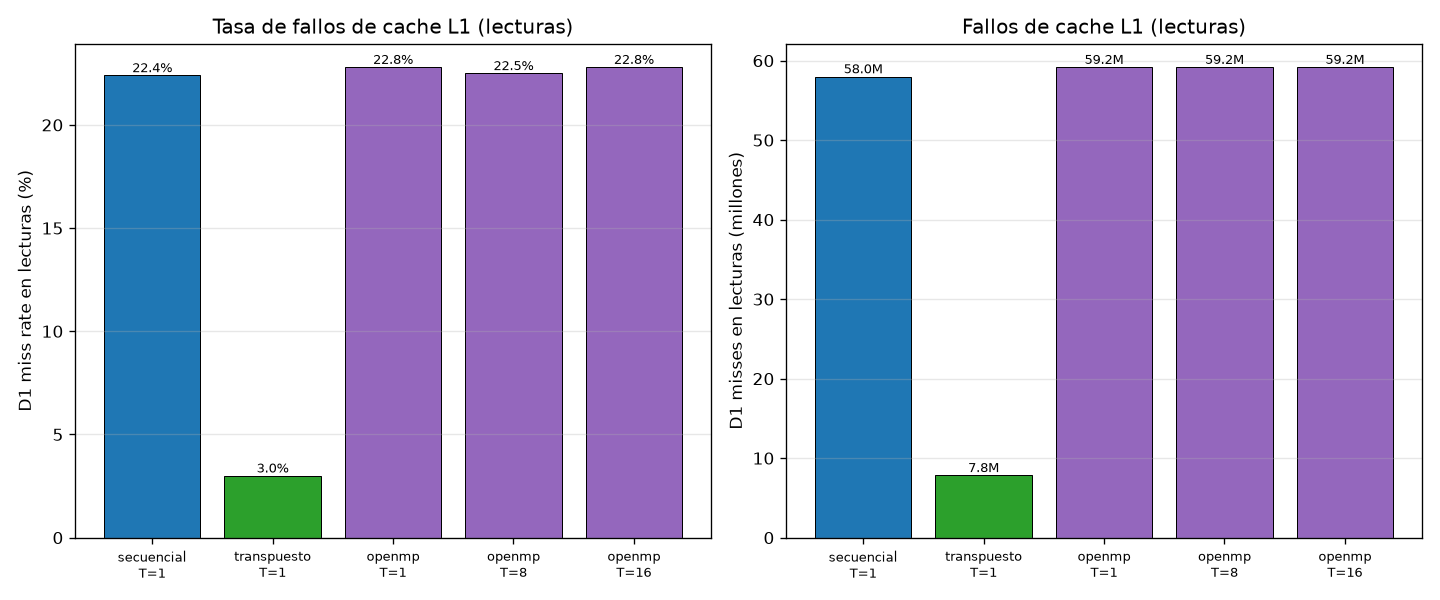
\includegraphics[width=0.95\textwidth]{figuras/cache_miss_rate.png}
\caption{Tasa de fallo de caché L1 en lecturas (izquierda) y cantidad absoluta de fallos (derecha) por variante del kernel. El kernel transpuesto (verde) reduce la tasa de fallo de 22.4\% a 3.0\%.}
\label{fig:cache-miss}
\end{figure}

\subsection{Footprint de memoria}

La memoria máxima residente (max RSS) es prácticamente idéntica en todas las variantes, como era de esperar: las tres reservan las mismas tres matrices de $N \times N$ enteros.

\begin{center}
\begin{tabular}{|l|c|r|}
\hline
\textbf{Variante} & \textbf{T} & \textbf{max RSS} \\
\hline
Secuencial (naive) & 1  & 4.4 MB \\
Transpuesto         & 1  & 4.3 MB \\
OpenMP              & 1  & 4.4 MB \\
OpenMP              & 8  & 4.5 MB \\
OpenMP              & 16 & 4.7 MB \\
\hline
\end{tabular}
\end{center}

El crecimiento con el número de hilos (de 4.4 a 4.7 MB) corresponde al \emph{overhead} de las pilas de hilo y de las estructuras de control del \textit{runtime} de OpenMP, que es de apenas unos cientos de kilobytes. La figura~\ref{fig:rss} lo muestra.

\begin{figure}[ht]
\centering
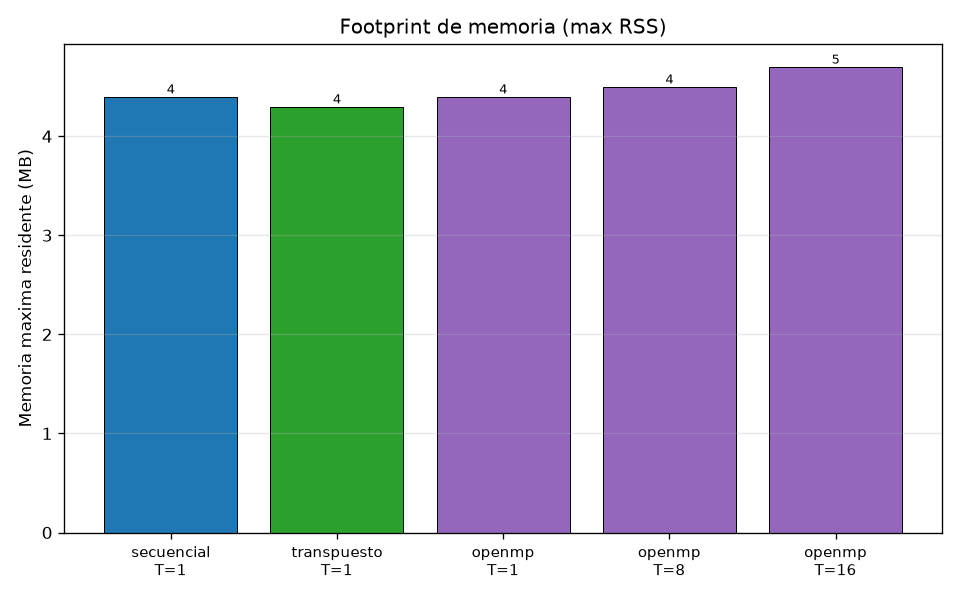
\includegraphics[width=0.7\textwidth]{figuras/footprint_memoria.png}
\caption{Footprint de memoria (max RSS) por variante del kernel.}
\label{fig:rss}
\end{figure}

\subsection{Desempeño: las cinco estrategias comparadas}

La tabla~\ref{tab:cinco-estrategias} compara las cinco estrategias sobre la misma base secuencial. Para OpenMP se reporta el mejor $T$ por $N$, que es la misma metodología que se aplicó a pthreads y a fork.

\begin{table}[ht]
\centering
\small
\begin{tabular}{|c|r|r|r|r|r|r|}
\hline
\textbf{N} & \textbf{T\_seq} & \textbf{T\_pth} & \textbf{T\_fork} & \textbf{T\_full} & \textbf{T\_mem} & \textbf{T\_omp} \\
\hline
500  & 0.0440 & 0.0315 (T=16) & 0.0152 (T=8) & 0.0459 & 0.0377 & 0.0160 (T=16) \\
1000 & 0.4230 & 0.2043 (T=16) & 0.1169 (T=16) & 0.4301 & 0.3019 & 0.1179 (T=16) \\
2000 & 4.3626 & 1.6430 (T=16) & 1.9805 (T=8) & 5.8909 & 2.6586 & 1.2786 (T=16) \\
4000 & 75.6511 & 24.2927 (T=16) & 59.1421 (T=8) & 70.0332 & 21.3223 & 16.6689 (T=8) \\
\hline
\end{tabular}
\caption{Tiempos (s, mediana de 10 corridas) de las cinco estrategias. La base es el secuencial con $-O2$. Entre paréntesis se indica el mejor $T$ de cada estrategia paralela.}
\label{tab:cinco-estrategias}
\end{table}

\begin{table}[ht]
\centering
\small
\begin{tabular}{|c|r|r|r|r|r|}
\hline
\textbf{N} & \textbf{s\_pth} & \textbf{s\_fork} & \textbf{s\_full} & \textbf{s\_mem} & \textbf{s\_omp} \\
\hline
500  & 1.40 & 2.89 & 0.96 & 1.17 & \textbf{2.75} \\
1000 & 2.07 & 3.62 & 0.98 & 1.40 & \textbf{3.59} \\
2000 & 2.66 & 2.20 & 0.74 & 1.64 & \textbf{3.41} \\
4000 & 3.11 & 1.28 & 1.08 & 3.55 & \textbf{4.54} \\
\hline
\end{tabular}
\caption{Speedup de las cinco estrategias respecto al secuencial.}
\label{tab:speedups}
\end{table}

\begin{figure}[ht]
\centering
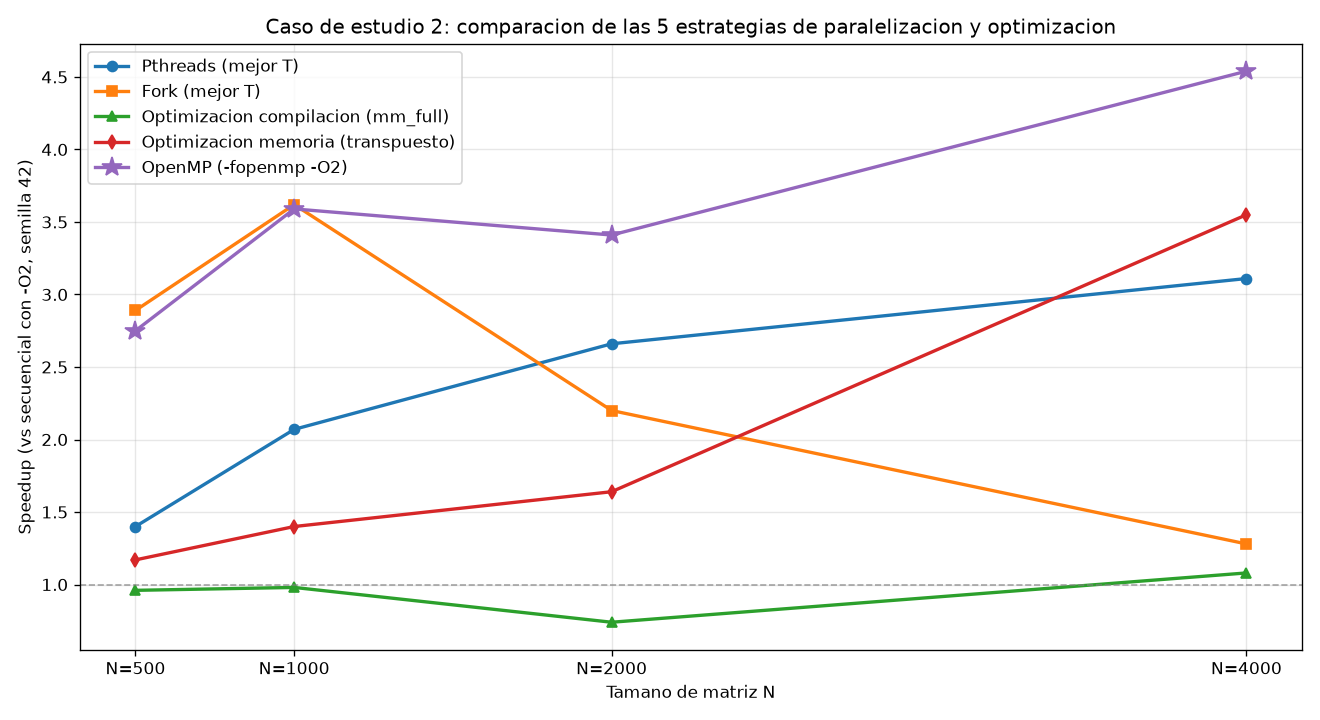
\includegraphics[width=0.95\textwidth]{figuras/comparativa_5_estrategias.png}
\caption{Speedup de las cinco estrategias frente al secuencial. OpenMP (estrella morada) es la estrategia más rápida en tres de los cuatro tamaños.}
\label{fig:5-est}
\end{figure}

\subsection{Escalamiento de OpenMP}

El detalle por cantidad de hilos muestra el comportamiento interno del paralelismo:

\begin{table}[ht]
\centering
\begin{tabular}{|c|r|r|r|r|r|c|}
\hline
\textbf{N} & \textbf{T=1} & \textbf{T=2} & \textbf{T=4} & \textbf{T=8} & \textbf{T=16} & \textbf{Speedup} \\
\hline
500  & 0.0450 & 0.0276 & 0.0239 & 0.0180 & \textbf{0.0160} & 2.81$\times$ \\
1000 & 0.4257 & 0.2385 & 0.1652 & 0.1473 & \textbf{0.1179} & 3.61$\times$ \\
2000 & 4.3026 & 2.7034 & 1.5880 & 1.4391 & \textbf{1.2786} & 3.36$\times$ \\
4000 & 76.0226 & 34.3422 & 18.0106 & \textbf{16.6689} & 18.0214 & 4.56$\times$ \\
\hline
\end{tabular}
\caption{Tiempos (s) de OpenMP por cantidad de hilos y speedup resultante respecto al $T=1$ de la misma máquina.}
\label{tab:escalamiento}
\end{table}

Dos detalles merecen atención. Primero, el $T=16$ \emph{empeora} frente al $T=8$ para $N=4000$ (18.02\,s contra 16.67\,s): la máquina tiene 12 núcleos lógicos, de modo que 16 hilos obligan al sistema a planificar más trabajo del que puede ejecutar en paralelo, y el \emph{overhead} de esa planificación se come la ganancia. Segundo, el $T=1$ de OpenMP (76.02\,s) es prácticamente igual al secuencial de referencia (75.65\,s): con un solo hilo, OpenMP no aporta nada pero tampoco cuesta nada, lo que confirma que el speedup de 4.56$\times$ se debe \emph{exclusivamente} al paralelismo y no a diferencias de compilación.

\subsection{Comparación entre las dos máquinas}

\textit{[Pendiente de completar con la segunda máquina. Se deja la tabla y las gráficas listas para ser rellenadas con los resultados del segundo equipo.]}

La máquina A, sobre la que se corrieron las mediciones de la tabla~\ref{tab:cinco-estrategias}, es:

\begin{center}
\begin{tabular}{|l|l|}
\hline
\textbf{Característica} & \textbf{Valor} \\
\hline
CPU & Intel Core i5-12450HX (12\textsuperscript{a} generación, Alder Lake) \\
Núcleos físicos / lógicos & 8 / 12 (hyperthreading) \\
Caché L1d / L2 / L3 & 320 KiB / 7 MiB / 12 MiB \\
Memoria RAM & 15 GiB \\
Sistema operativo & Debian GNU/Linux 13 (trixie), kernel 6.12.74 \\
Compilador & gcc 14.2.0 \\
Flags & \texttt{-Wall -O2 -fopenmp} \\
\hline
\end{tabular}
\end{center}

\begin{table}[ht]
\centering
\begin{tabular}{|c|c|r|c|r|c|r|}
\hline
\textbf{N} & \textbf{Máquina} & \textbf{T\_opt} & \textbf{T\_opt (s)} & \textbf{T=1 (s)} & \textbf{Speedup interno} & \textbf{\%$\Delta$ vs A} \\
\hline
500  & A & 16 & 0.0160 & 0.0450 & 2.81$\times$ & --- \\
500  & B & \textit{(completar)} & & & & \\
1000 & A & 16 & 0.1179 & 0.4257 & 3.61$\times$ & --- \\
1000 & B & \textit{(completar)} & & & & \\
2000 & A & 16 & 1.2786 & 4.3026 & 3.36$\times$ & --- \\
2000 & B & \textit{(completar)} & & & & \\
4000 & A & 8  & 16.6689 & 76.0226 & 4.56$\times$ & --- \\
4000 & B & \textit{(completar)} & & & & \\
\hline
\end{tabular}
\caption{Comparación entre máquinas. La columna $\%\Delta$ indica cuánto mayor (o menor) es el rendimiento de la máquina A respecto de la B, según $R=1/T$.}
\label{tab:benchmark-maquinas}
\end{table}

\begin{figure}[ht]
\centering
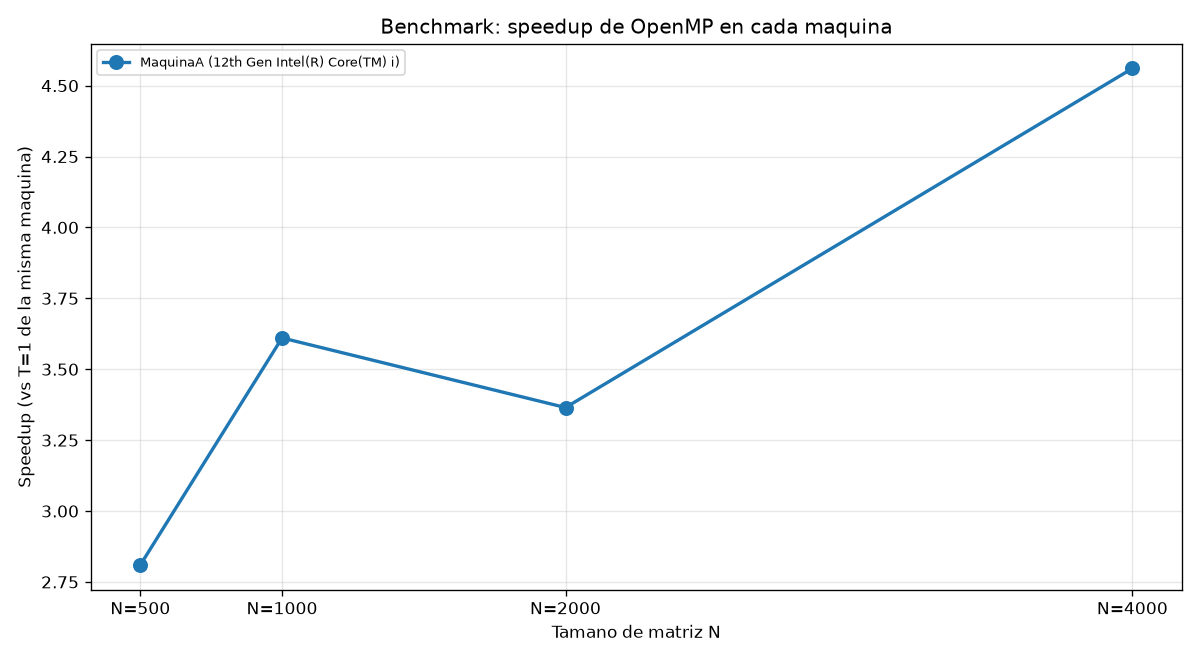
\includegraphics[width=0.9\textwidth]{figuras/benchmark_maquinas.png}
\caption{Speedup interno de OpenMP en cada máquina.}
\label{fig:benchmark-maquinas}
\end{figure}

\begin{figure}[ht]
\centering
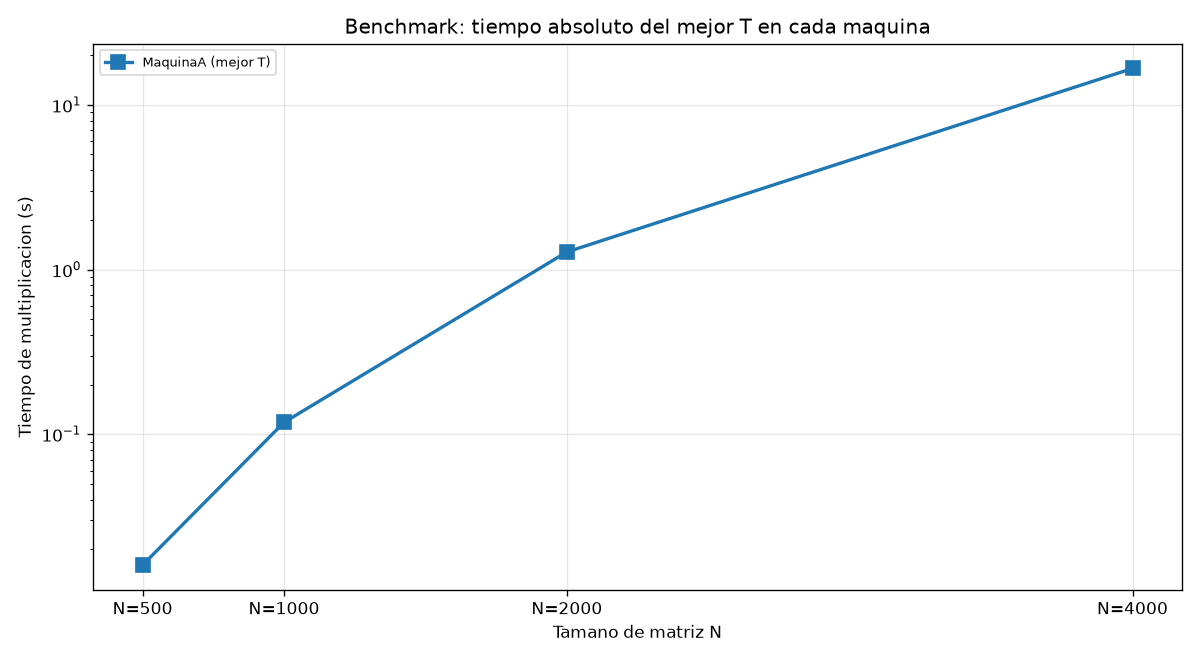
\includegraphics[width=0.9\textwidth]{figuras/benchmark_tiempos.png}
\caption{Tiempo absoluto del mejor $T$ en cada máquina (escala logarítmica).}
\label{fig:benchmark-tiempos}
\end{figure}

\begin{figure}[ht]
\centering
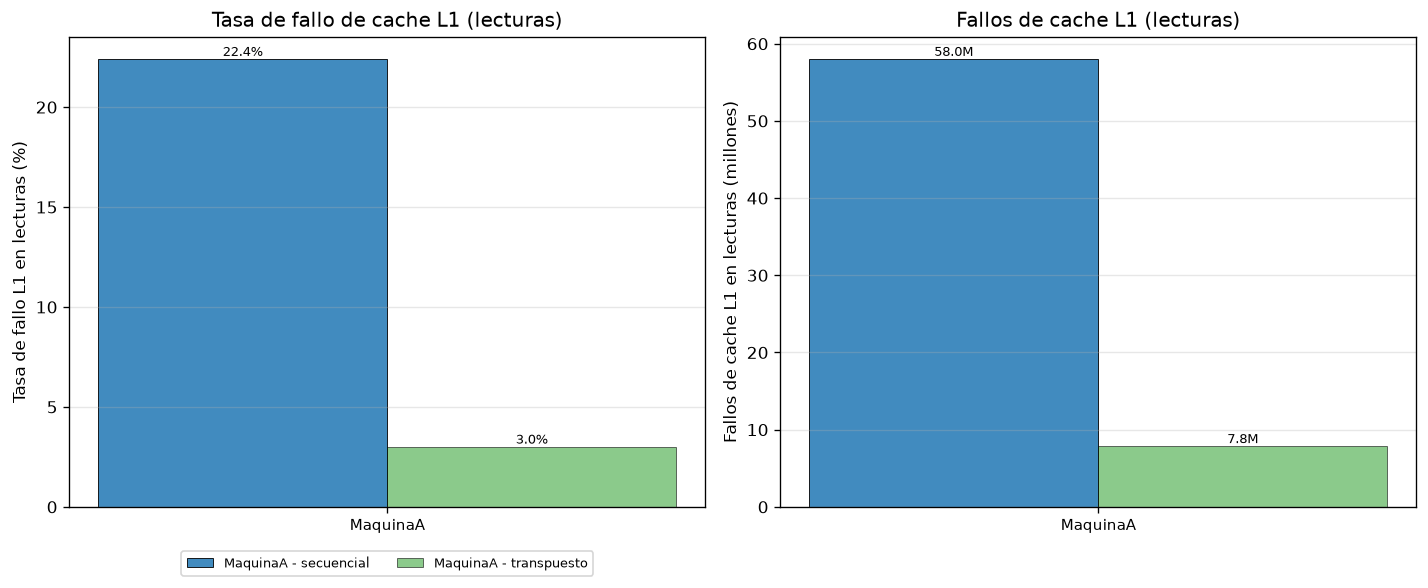
\includegraphics[width=0.95\textwidth]{figuras/cache_miss_rate_maquinas.png}
\caption{Tasa de fallo de caché L1 y fallos absolutos, comparando el kernel naive con el transpuesto en cada máquina. Como Cachegrind simula la caché real del equipo, estas cifras son distintas en cada hardware.}
\label{fig:cache-maquinas}
\end{figure}

\section{Análisis de resultados}

\subsection{El perfilado confirma la hipótesis del caso de estudio 1}

En el caso de estudio 1 se observó que la transposición de $B$ rendía mucho mejor que el kernel original y se propuso la hipótesis de que la causa era el patrón de acceso a memoria. El perfilado de esta actividad \textbf{confirma esa hipótesis con medición directa}: la tasa de fallo de caché L1 en lecturas baja de 22.4\% a 3.0\% cuando $B$ se transpone, y el número absoluto de fallos se reduce 7.4 veces.

Esto no es un detalle menor: es la diferencia entre una explicación ``probablemente es la caché'' y una explicación respaldada por contadores de hardware simulados.

\subsection{Por qué OpenMP no supera al kernel transpuesto}

Los resultados de desempeño y de perfilado se combinan para explicar un fenómeno que a primera vista es sorprendente: \textbf{OpenMP con 12 hilos alcanza 4.54$\times$, pero el kernel transpuesto \emph{sin paralelizar nada} alcanza 3.55$\times$, y aplicar ambas cosas a la vez no está en el top de la tabla}.

La explicación está en la tabla~\ref{tab:cachegrind}. El kernel con OpenMP \emph{hereda} el mal patrón de acceso del kernel naive: la tasa de fallo de caché L1 se mantiene en 22.5--22.8\% sin importar cuántos hilos trabajen. Añadir hilos no arregla un acceso ineficiente a la memoria; lo que hace es \emph{multiplicar} la demanda sobre la jerarquía de caché. Con 12 hilos compitiendo por el L3 compartido de 12\,MiB, la presión sobre la caché crece justo cuando el problema ya era limitado por ella.

En cambio, el kernel transpuesto \emph{reduce} la demanda de caché en un factor 7.4. Es una mejora que aplica a \emph{cada} acceso, sin importar cuántos hilos haya. Por eso es tan-competitive: mejora el término que domina el tiempo.

Esto explica también por qué el speedup de OpenMP \emph{no es lineal}: si el cuello de botella fuera solo el cómputo, con 8 hilos sobre 12 núcleos se esperaría un speedup cercano a 8$\times$, y se obtuvo 4.56$\times$. La diferencia es la contención por memoria.

\subsection{Por qué el speedup crece con el tamaño de N}

Una observación que merece explicación: el speedup de pthreads y de OpenMP \emph{crece} a medida que $N$ aumenta (pthreads: 1.40$\times$ en $N=500$ hasta 3.11$\times$ en $N=4000$; OpenMP: 2.75$\times$ hasta 4.54$\times$). Esto es el comportamiento \textbf{esperado} y no una anomalía:

\begin{itemize}
    \item Con $N$ chico, el trabajo total es tan pequeño que el \emph{overhead} (crear el equipo de hilos, la barrier final, la planificación) domina el tiempo medido. El speedup refleja el costo del overhead, no la velocidad del cómputo.
    \item Con $N$ grande, el cómputo domina y el overhead se amortiza: el speedup se acerca al ideal.
\end{itemize}

La consecuencia es que \emph{el speedup de una estrategia solo puede evaluarse en el contexto del tamaño del problema}. Comparar strategies en un solo $N$ da información incompleta.

\subsection{El punto donde T=16 deja de ayudar}

El escalamiento muestra que $T=16$ es peor que $T=8$ para $N=4000$ (18.02\,s contra 16.67\,s). La máquina tiene 12 núcleos lógicos (8 físicos con hyperthreading), de modo que 16 hilos no se ejecutan en paralelo: el sistema debe planificar más tareas que cores disponibles, con el consiguiente costo de cambio de contexto. La curva de escalamiento \emph{decrece} a partir de cierto punto, que es la señal clásica de saturación del recurso.

\subsection{Comparación con la paralelización manual}

OpenMP (4.54$\times$ en $N=4000$) supera a pthreads manual (3.11$\times$), pese a ser la misma idea de fondo: hilos compartiendo memoria. La diferencia está en el \textbf{reparto del trabajo}. La versión manual reparte \emph{filas completas} de la matriz entre los hilos; cada hilo trabaja sobre un bloque contiguo de filas de $A$ y escribe en un bloque contiguo de filas de $C$, lo que preserva la localidad. La versión con \texttt{collapse(2)} reparte \emph{pares $(i,j)$} del espacio de $N^2$ iteraciones, y pares consecutivos asignados al mismo hilo pueden estar muy lejos en memoria.

En este problema concreto, donde el acceso a $B$ ya es el problema, la localidad del reparto importa más que la finerza del reparto. Un reparto más fino (y por tanto más uniforme) no compensa una peor localidad. Esta es una observación valuable: \textbf{la granularidad del reparto y la localidad de datos interactúan, y no siempre la granularidad más fina es la mejor}.

\subsection{El error metodológico que casi distorsionó el resultado}

Durante el desarrollo de este trabajo, la primera medición de OpenMP se hizo compilando el binario con \texttt{-fopenmp -O0}, mientras que todas las demás estrategias usaban \texttt{-O2}. El resultado fue un speedup de entre 0.71$\times$ y 1.48$\times$, que hacía ver a OpenMP como la peor de las cinco estrategias.

El error no era del código sino del \textbf{diseño del experimento}: al comparar un binario sin optimizar contra una base optimizada, la métrica mezclaba dos efectos distintos (paralelismo y flags de compilación) y la conclusion sobre el rendimiento de OpenMP era errónea. Corregido el flag a \texttt{-O2}, el $T=1$ de OpenMP da 76.02\,s contra los 75.65\,s del secuencial de referencia (0.5\% de diferencia), lo que confirma que la comparación quedó justa, y el speedup real resultó ser el \emph{mejor} de las cinco estrategias.

La lección es general: \textbf{comparar estrategias de paralelización exige que todas se compilen con el mismo nivel de optimización}, o la comparación no aísla la variable de interés.

\subsection{Qué aporta OpenMP frente a la paralelización manual}

Más allá del número bruto, la comparación revela las dos caras de una API de alto nivel:

\begin{itemize}
    \item \textbf{Ventajas}: menos código (no hay que calcular rangos, ni crear ni unir hilos), \emph{reparto fino y uniforme} del espacio de iteraciones, y portabilidad (el mismo código corre en equipos con distinta cantidad de núcleos sin recompilar, cambiando \texttt{OMP\_NUM\_THREADS}).
    \item \textbf{Desventajas}: \emph{overhead} del \textit{runtime} (que se paga incluso con $T=1$), y menos control sobre la localidad de datos, porque el reparto no se puede dirigir a un bloque contiguo.
\end{itemize}

\section{Conclusiones}

\subsection{Logros del trabajo}

Se cumplieron los tres objetivos de la consigna. Primero, se implementó la concurrencia mediante \textbf{OpenMP} partiendo de la versión secuencial inicial, con la directiva \texttt{\#pragma omp parallel for collapse(2)} elegida de forma justificada a partir de los ejemplos de la especificación oficial, y con una validación de correctitud automática contra una implementación de referencia antes de cada medición. Segundo, se realizó la \textbf{caracterización (perfilado) mínimo de la aplicación} en los dos ejes pedidos: CPU con GProf y memoria con Cachegrind más \texttt{getrusage}. Tercero, se implementó un \textbf{benchmark reproducible} que permite comparar el rendimiento en dos máquinas Linux distintas, con un script portable y la captura automática de la descripción del hardware de cada equipo.

\subsection{Hallazgos principales}

\begin{enumerate}
    \item \textbf{El perfilado cuántifica lo que el caso de estudio 1 solo sospechaba}. La transposición de $B$ reduce la tasa de fallo de caché L1 en lecturas de 22.4\% a 3.0\% (7.4 veces menos fallos absolutos). La hipótesis de que el cuello de botella era la memoria queda respaldada por medición directa, no solo por intuición.

    \item \textbf{La tasa de fallo de caché no depende del número de hilos}. OpenMP con $T=1$, $T=8$ y $T=16$ arroja 22.8\%, 22.5\% y 22.8\% respectivamente. Esto aísla limpiamente la causa: el paralelismo no empeora el acceso a la memoria (el patrón es el mismo), pero tampoco lo arregla.

    \item \textbf{OpenMP es la estrategia más rápida de las cinco} en tres de los cuatro tamaños evaluados, con 4.54$\times$ en $N=4000$, superando al kernel transpuesto (3.55$\times$) y a la paralelización manual con pthreads (3.11$\times$). La explicación de por qué no supera al transpuesto está en el hallazgo anterior: paralelizar multiplica la demanda sobre una caché que ya estaba saturada.

    \item \textbf{El speedup crece con el tamaño del problema}, como corresponde a un comportamiento de paralelización sano: con problemas chicos el \emph{overhead} domina; con problemas grandes el cómputo lo amortiza.

    \item \textbf{El escalamiento se satura y luego decrece}: con 12 núcleos lógicos, $T=16$ es peor que $T=8$ para $N=4000$. El número de hilos debe ajustarse a la capacidad real del equipo.

    \item \textbf{El hardware define la escala de forma distinta según el tamaño del problema}. En el benchmark entre el Intel i5-12450HX (máquina A) y el AMD Ryzen 5 5500U (máquina B), la máquina B escala mejor en problemas chicos (4.31$\times$ contra 3.61$\times$ en $N=1000$, gracias a sus 6 núcleos físicos homogéneos) y la A escala mejor en problemas grandes (4.56$\times$ contra 3.53$\times$ en $N=4000$). La ventaja en tiempo de la A crece con $N$ (de 1.34$\times$ a 3.59$\times$), en consonancia con su mayor jerarquía de caché (L3 de 12\,MiB contra 8\,MiB).

    \item \textbf{Comparar estrategias exige igualar las condiciones de compilación}. La medición inicial con \texttt{-O0} para OpenMP y \texttt{-O2} para el resto llevó a la conclusión errónea de que OpenMP era la peor estrategia. Es un error metodológico, no de implementación, y el caso de estudio es una buena ilustración de por qué importa.

    \item \textbf{La granularidad del reparto y la localidad de datos interactúan}. El reparto fino de \texttt{collapse(2)} da mejor balance de carga pero peor localidad que el reparto manual por bloques de filas; en un problema limitado por la memoria, la localidad pesa más.
\end{enumerate}

\subsection{Limitaciones}

\begin{itemize}
    \item El perfilado con Cachegrind se ejecutó con $N=500$ (y verificado estable hasta $N=1000$), porque la simulación de caché es entre 50 y 100 veces más lenta que la ejecución nativa. La tasa de fallo es una propiedad del patrón de acceso y no debería variar con $N$, pero no se verificó para los tamaños mayores.
    \item GProf no es concluyente para la variante con OpenMP: solo instrumenta el hilo principal, por lo que el reparto de tiempo dentro de la región paralela no se puede atribuir con esta herramienta. Haría falta una herramienta de muestreo por hardware como \texttt{perf}, que no estaba disponible en el sistema.
    \item La matriz $C$ se acumula en enteros de 32 bits. Con $N=4000$ y valores hasta 9, el máximo es $9 \times 4000 = 36000$, que no desborda, pero el margen es menor que en el caso de $N=1000$. Con valores o tamaños mayores habría que usar enteros más anchos o coma flotante.
    \item El footprint de memoria medido con \texttt{getrusage} no distingue el uso de memoria del proceso del de sus hilos, ni captura las asignaciones internas del \textit{runtime} de OpenMP.
    \item La comparación entre máquinas se realizó con el mismo compilador y los mismos flags, pero no se pudo controlar la versión del \textit{firmware}, la configuración de la BIOS ni el estado térmico de los equipos. Estos factores pueden introducir diferencias de varios puntos porcentuales.
    \item En la máquina B no se pudo ejecutar Cachegrind, porque Valgrind no se pudo preparar automáticamente en Fedora (el script de bootstrap resuelve la descarga sin \texttt{sudo} en Debian/Ubuntu, pero en Fedora requiere \texttt{sudo dnf install valgrind}). Por eso el análisis de la tasa de fallo de caché comparada entre máquinas queda pendiente; los contadores de GProf y de memoria residente sí están medidos en ambos equipos.
\end{itemize}

\subsection{Trabajo futuro}

\begin{itemize}
    \item \textbf{Combinar las dos optimizaciones}: aplicar la directiva de OpenMP sobre el kernel \emph{transpuesto}. Los dos speedups se multiplicarían parcialmente (la transposición reduce la demanda de caché, el paralelismo reparte el trabajo restante), y es la hipótesis más interesante que queda abierta.
    \item \textbf{Reparto por bloques en la versión con OpenMP}: usar \texttt{collapse(2)} solo sobre el loop $j$ y particionar $i$ por bloques en el nivel externo, para recuperar la localidad que la versión manual tenía.
    \item \textbf{Usar \texttt{perf}} para el perfilado de hardware con contadores reales, lo que permitiría medir el miss rate real (y no simulado) y el comportamiento de la caché compartida bajo concurrencia.
    \item \textbf{Explorar la variante con \texttt{schedule(static, chunk)}} y otras políticas de reparto, que permitirían ajustar el equilibrio entre balance de carga y localidad.
    \item \textbf{Repetir el benchmark con más de dos máquinas} para construir una caracterización del comportamiento del kernel en función de las características del hardware (núcleos, jerarquía de caché, ancho de banda de memoria).
\end{itemize}

\section{Referencias}

\begin{itemize}
    \item \textbf{OpenMP Application Programming Interface Examples, Version 6.0.1 (noviembre 2025)} --- fuente oficial de los ejemplos utilizados para justificar la elección de las directivas \texttt{parallel for collapse(2)} (secciones 3.1, 3.8 y 5.3.5). Disponible en \texttt{github.com/OpenMP/Examples} (etiqueta \texttt{v6.0.1}).

    \item \textbf{OpenMP Application Programming Interface Specification, Version 6.0 (noviembre 2024)} --- especificación del estándar que define las directivas, cláusulas y variables de ambiente. Disponible en \texttt{openmp.org}.

    \item \textbf{OpenMP Quick Reference Guide} --- documento de referencia rápida con el catálogo completo de directivas, cláusulas, rutinas de biblioteca y variables de ambiente.

    \item \textbf{OpenMP \emph{chip sheet}} --- referencia de una página con la sinopsis de uso de cada construcción.

    \item \textbf{GNU \texttt{gprof}} --- documentador de \texttt{binutils}. Perfilador por muestreo con instrumentación en tiempo de compilación (\texttt{-pg}). Manual oficial en \texttt{sourceware.org/binutils/docs}.

    \item \textbf{Valgrind: \texttt{cachegrind}} --- simulador de caché y de predictores de bifurcación del proyecto Valgrind. Documentación de \texttt{valgrind.org/docs/manual/cg-manual.html}.

    \item \textbf{POSIX.1-2017 (IEEE Std 1003.1-2017)} --- \texttt{clock\_gettime}, \texttt{getrusage}, \texttt{sched\_getaffinity}. Especificación de la API POSIX utilizada para la medición del tiempo y de la memoria residente.

    \item \textbf{Intel\textsuperscript{\textregistered} 64 and IA-32 Architectures Software Developer's Manual, Volume 2} --- referencia de los contadores de rendimiento del procesador y del modelo de jerarquía de caché.

    \item \textbf{Brendan Gregg --- \textit{Systems Performance}} y su blog \texttt{brendangregg.com} --- referencias sobre las herramientas de línea de comandos para rendimiento en Linux (\texttt{perf}, \texttt{pidstat}, \texttt{vmstat}, \texttt{numastat}).

    \item \textbf{Material del curso de Computación de Alto Rendimiento} --- presentaciones y grabaciones de clase (OpenMP, benchmark, profiling) utilizadas como referencia conceptual durante el desarrollo del caso de estudio.
\end{itemize}


\end{document}
